\documentclass{article}
\usepackage[lmargin=2.54cm, rmargin=2.54cm,tmargin=2.54cm,bmargin=2.54cm]{geometry}
\usepackage{doc}
\usepackage{graphicx}
\usepackage{indentfirst}
\usepackage{setspace}

\title{Homework 2}
\author{Anthony Menjivar}

\date{March 3rd 2015}

\begin{document}

\maketitle

\section{Problem 0.1}
a) $f(n) = n - 100$ $g(n) = n - 200$	

$f = \Theta(g)$

b) $f(n) = n^{1/2}$ $g(n) = n^{2/3}$   

$f = O(g)$

c) $f(n) = 100n + logn$ $g(n) = n + (logn)2$

$f = \Theta(g)$

d) $f(n) = n(logn)$ $g(n) = 10n(logn) $

$f = \Theta(g)$

e) $f(n) = log2n$ $g(n) = log3n$

$f = \Theta(g)$

f) $f(n) = 10(logn)$ $g(n) = log(n^{2})$ 

$f = \Theta(g)$

g) $f(n) = logn^{1.01}$ $g(n) = n(log^{2}n)$  

$f = \Omega(g)$

h) $f(n) = \frac{n^{2}}{logn}$ $g(n) = n(logn)^{2}$

$f = Omega(g)$

i) $f(n) = n^{0.1}$ $g(n) = (logn)^{10}$ 

$f = \Omega(g)$ 

j) $f(n) = (logn)^{logn}$ $g(n) = \frac{n}{logn}$

$ f = \Omega(g)$

k) $f(n) = \sqrt{n}$ $g(n) = (logn)^{3}$ 

$f = \Omega(g)$

l) $f(n) = n^{1/2}$ $g(n) = 5^{log_{2}n}$ 

$f = 0(g)$

m) $f(n) = n2^{n}$ $g(n) = 3^{2}$ 

$f = O(g)$

n) $f(n) = 2^{n}$ $g(n) = 2^{n+1}$ 

$f = \Theta(g)$

o) $f(n) = n!$ $g(n) = 2^{n}$ 

$f = \Omega(g)$

p) $f(n) = (logn)^{logn}$ $g(n) = 2^{(log_{2}n)^{2}}$ 

$f = O(g)$

q) $f(n) = \Sigma^{n}_{i=1}i^{k}$ $g(n) = n^{k+1}$ 

$f = \Theta(g)$

\section{Problem 0.4}
Is there a faster way to compute the nth Fibonacci number than by fib2 (page 13)? One idea
involves matrices.

We start by writing the equations F1 = F1 and F2 = F0 + F1 in matrix notation:

\begin{center}
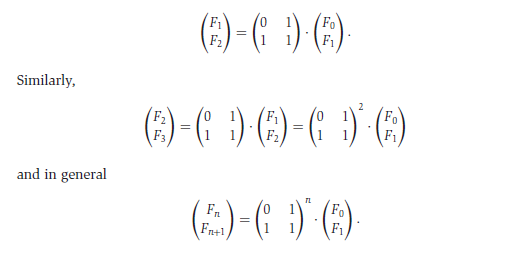
\includegraphics{Screenshot(169)}
\end{center}

So in order to computer $F_{n}$, it suffices to raise this 2 x 2 matrix, call it $X$, to the $n$th power. 
\subsection{Problem 0.4(a)}
Show that two 2 x 2 matrices can be multiplies using 4 additions and 8 multiplications.
\vspace{2mm}

Considering any 2 x 2 matrices, for example 2 x 2 matrices X and Y. We can look at the same matrices above. Every entry of XY is the addition of 2 products of the entries. Therefore each can be computed in 2 multiplactions and one addition. Since this is a 2 x 2 matrix, it can be calculated in 4 multiplications and 4 additions.
\subsection{Problem 0.4(b)}
But how many matrix manipulations does it take to compute $X^{n}$? Show that $O(logn)$ matrix multiplication suffice for computing $X^{n}$.
\vspace{2mm}

Considering the case of $n = 2^{k}$ for some positive integer k. To compute, $X^{2^{k}}$, we can compute $Y = X^{2^{k-1}}$ and from there we can compute to get $Y^{2} = X^{2^{k}}$ by squaring. Doing this recursively we get $X^{2}, X^{4},...,X^{2^{k}} = X^{^{n}}$. Each time we are doubling the exponent of $X$ meaning that it must take $k = logn$ matrix multiplications to produce $X^{n}$. Therefore this still requires $O(logn)$ matrix manipulations. 

\section{Problem 1.2}
Show that any binary integer is at most four times as long as the corresponding decimal integer.
For very large numbers, what is the ratio of these two lengths, approximately?
\vspace{2mm}

Considering a number N. In binary we need $\lceil log_{2}N+1 \rceil$ digits while in decimal we need $\lceil log_{2}(N+1) \rceil$ digits.

\begin{center}
$\lceil log_{10}N+1 \rceil$

=

$\lceil log_{2}(N+1) *\, log_{2}(10) \rceil$ $\leq$ $\lceil log_{2}(10) \rceil *\, \lceil log_{2}(10) \rceil$ = $4 *\, \lceil log_{2}(N+1)\rceil$

$\lceil log_{2}(N+1) *\, log_{2}(10) \rceil$ $\approx$ $log_{2}(N+1)$ $\approx$ $3.8$
\end{center}

The ration is approximately 3.8 between the two lengths and this shows that there are at most 4 times the amount of digits in binary.

\section{Problem 1.4}
Show that: $log(n!)$ $=$ $\Theta(nlogn)$
\vspace{2mm}

\begin{center}
$log(n!) = log(1) + log(2) + ... + log(n-1) + log(n)$

Upper Bound: $log(1) + log(2) + ... + log(n) \leq log(n) + log(n) + ... log(n) = nlogn$

Get the lower bound by doing the same thing and then we get:

$log(1) + ... + log(\frac{n}{2}) + ... + log(n) \geq log(\frac{n}{2}) + ... + log(n) \geq log(\frac{n}{2}) + ... + log(\frac{n}{2}) = \frac{n}{2} log(\frac{n}{2})$
\end{center}

\section{Problem 1.11}
Is $4^{1536} - 9^{4824}$ divisible by 35?
\vspace{2mm}

Since 35 is prime, using Fermat's Little Theorem:
\begin{center}
$35 = 5 *\, 7$

$a^{(5-7)*(7-1} = a^{4*6} = a^{2}4 \equiv$ 1 $mod$ $35$ when $1 \leq a < 35$ 
\vspace{2mm}

$4^{1536} = 4^{24*64} \equiv$ 1 $mod$ $35$ and,

$9^{4824} = 9^{24*201} \equiv$ 1 $ mod$ $35$
\vspace{2mm}
\end{center}

Therefore, $4^{1536} \equiv 9^{4824}$ and the difference is divisible by 35.

\section{Problem 1.13}
Is the difference of $5^{30,000}$ and $6^{123,456}$ a multiple of 31?
\vspace{2mm}

Since 31 is prime, using Fermat's Little Theorem:

\begin{center}
$a^{30} \equiv 1$ $mod$ 31 when $1 \leq a < 31$

Therefore, $5^{30,000} \equiv 1$ $mod$ 31
\vspace{2mm}

$6^{123456} = 6^{123450 + 6}$ $\rightarrow$ $6^{6}$

$5^{3} = 125$ $mod$ 31 $\equiv$ 1 $mod$ 31
\end{center}

Therefore the difference of $5^{30,000}$ and $6^{123,456}$ is a multiple of 31.

\section{Problem 1.16}
The algorithm for computing $a^{b}$ mod c by repeated squaring does not necessarily lead to the
minimum number of multiplications. Give an example of b $>$ 10 where the exponentiation can
be performed using fewer multiplications, by some other method.
\vspace{2mm}

\begin{center}
Let b = 15

Repeated Squaring: $a, a^{2}, a^{4}, a^{8}$ $\Rightarrow$ $a^{15} = a *\, a^{2} *\, a^{4}*\, a^{8}$ which is a total of 6 multiplications
\vspace{2mm}

$a^{3} = a *\, a *\, a$ and $a^{12} = a^{6} *\, a^{6}$
Now we can calculate $a^{15} = a^{12} *\, a^{3}$ which is a total of 5 multiplications
\end{center}

\section{Problem 1.25}
Calculate $2^{125}$ mod 127 using any method you choose.

\begin{center}
127 is odd, using Fermat's Little Theorem...

$42^{126} \equiv$ 1 mod 127 

$2^{126} = 2^{125}$

$2^{125}$ is the inverse of 2 mod 127

2 * 64 = 128 $\equiv$ 1 mod 127

$2^{125} =$ 64 mod 127 since it is a unique inverse
\end{center}

\section{Problem 1.33}
Give an efficient algorithm to compute the least common multiple of two n-bit numbers x and
y, that is, the smallest number divisible by both x and y. What is the running time of your
algorithm as a function of n?
\vspace{2mm}

The LCM can be found using the greatest common divisor as seen in the equation $lcm(x,y) = \frac{x*y}{gcd(x,y)}$. Because we need $O(n^{2})$ operations to multiply $x$ and $y$ and $O(n^{2})$ operations to divide, the total running time for this algorithm would be $O(n^{3})$.

\section{Problem 1.35(d)}
Unlike Fermat’s Little theorem, Wilson’s theorem is an if-and-only-if condition for primality.
Why can’t we immediately base a primality test on this rule?
\vspace{2mm}

The running time of the algorithm would not be efficient in this case because depending on the size of whatever number N in a factorial product would take exponential time.

\section{Problem 1.39}
Give a polynomial-time algorithm for computing $a^{b^{c}}
mod$ p, given a, b, c, and prime p.
\vspace{2mm}

Using Fermat's Little Theorem: $a^{p-1} = 1$ mod p. Therefore $a^{b^{c}} mod p - a^{b^{c} mod (p-1)} mod$ p

First: $(b mod (p-1))$ in time $O(logb*logp)$

Second: Compute $(b^{c} mod (p-1))$ using repeated squared. Each multiplication will take $O(log^{3}p)$ for a total time of $O(logc*log^{2}p)$

Third: $(a mod p)$ in time $O(loga*logp)$

Fourth: Using repeated squaring to compute $(a^{b^{c}} mod p)$ it takes $O(logp*log^{2}p) - O(log^{3}p)$
\vspace{2mm}

Total running time: $O(logb * logp + logc * log^{2}p + loga * logp + log^{3}p)$ which is upper bounded by $O(n^{3})$
\end{document}
